\documentclass{article}
\usepackage[utf8]{inputenc}
\usepackage[T1]{fontenc}
\usepackage[croatian]{babel}
\usepackage{placeins}
\usepackage{mathptmx}
\usepackage{amsmath}
\usepackage{amssymb}
\usepackage{siunitx}
\usepackage{graphicx}
\usepackage[sorting=none]{biblatex}
%\addbibresource{literatura.bib}

\numberwithin{figure}{section}
\numberwithin{table}{section}

\begin{document}

\begin{titlepage}
	\centering
	{\scshape\LARGE Sveučilište u Zagrebu\par}
	\vspace{0.5cm}
	{\scshape\Large Fakultet elektrotehnike i računarstva\par}
    \vfill
	{\Large\itshape Projekt kolegija Ekspertni sustavi \par}
	\vspace{0.5cm}
	{\huge\bfseries Rješavanje i analiza rješavanja igrice Minesweeper\par}
	\vspace{0.5cm}
	{\Large\itshape Darko Janeković, Jelena Nemčić \par}
	\vfill
	{\large Zagreb, 2020.}
\end{titlepage}

\section{Uvod}

Minesweeper je igra za jednog igrača koja se sastoji od ploče dimenzija $X \times Y$. Neka od polja ploče sadrže skrivene mine, a igračev je cilj locirati sve mine i otvoriti sva preostala polja.

Igraču je u svakom trenutku igre poznato koliko je mina još na ploči. U svakom svom potezu igrač može:
\begin{itemize}
    \item označiti polje kao da se tamo nalazi mina,
    \item maknuti oznaku mine s prethodno označenog polja,
    \item otvoriti polje.
\end{itemize} 

Označavanjem polja kao mine smanjuje se broj preostalih mina neovisno o tome nalazi li se stvarno mina na tom polju. Ukoliko je polje označeno kao mina nije ga moguće otvoriti bez da se prethodno makne oznaka da se tamo
nalazi mina. Takva akcija označavanja je korisna ukoliko igrač sa sigurnošću zna da se na nekom polju
nalazi mina. S druge strane, igrač može otvoriti polje oko kojeg se ne nalazi niti jedna
mina, polje oko kojeg se nalazi $n$ mina te konačno polje na kojem se nalazi mina.

Otvaranje polja oko kojeg se ne nalazi niti jedna mina nastavit će rekurzivno otvarati susjedna
polja sve dok se ne otvori neko polje koje u susjedstvu ima minu. Otvaranje polja oko kojeg
se nalazi $n$ mina ispisat će na ploču brojku $n$. Igrač je izgubio ako je otvorio polje s minom, dok otvaranje zadnjeg polja koje nije mina
označava pobjedu.

U okviru ovog projekta bit će analizirane dvije taktike za rješavanje igrice Minesweeper pri čemu obje
taktike svode problem na programiranje s ograničenjima (engl. \textit{Constraint Programming}),
ali se postupak rješavanja razlikuje.

U prvom slučaju problem će se rješavati simpleks metodom, dok će se u drugom slučaju isti
problem rješavati i tretirati kao problem zadovoljivosti (engl. \textit{Satisfaction Problem}).
Prednosti i nedostatci oba načina rješavanja bit će komentirani u nastavku.

\section{Modeliranje problema}

Moguće je pretpostaviti, bez gubitka općenitosti, da je ploča dimenzija $3 \times 3$ te da je
svaka vrijednost na ploči $m_{i, j} \in \{\bot, \top\}$. Ukoliko je vrijednost pojedinog polja
$\top$ tamo se nalazi mina, odnosno ako je vrijednost $\bot$ na tom se polju ne nalazi mina.
Skup $\mathcal{N}(m_{i, j})$ definira susjedstvo polja $m_{i, j}$, a s $n$ će biti označavan broj mina
u susjednim poljima polja $m_{i, j}$, pri čemu se gledaju sva polja koja su mu susjedna horizontalno, vertikalno i dijagonalno.

Nakon otvaranja polja $m_{i, j}$ agent u bazu znanja upisuje:
\begin{equation}
    \sum_{a \in \mathcal{N}(m_{i, j})} a = n
    \label{eq:1}
\end{equation}

\subsection{Zaključivanje}
Zaključivanje korištenjem ranije definiranih pravila bit će objašnjeno u nastavku. Stanje
svijeta prikazano je tablicom:

\begin{table}[ht]
    \centering
    \begin{tabular}{llll}
                           & 1                      & 2                      & 3                      \\ \cline{2-4}
    \multicolumn{1}{l|}{1} & \multicolumn{1}{l|}{}  & \multicolumn{1}{l|}{}  & \multicolumn{1}{l|}{}  \\ \cline{2-4}
    \multicolumn{1}{l|}{2} & \multicolumn{1}{l|}{1} & \multicolumn{1}{l|}{1} & \multicolumn{1}{l|}{1} \\ \cline{2-4}
    \multicolumn{1}{l|}{3} & \multicolumn{1}{l|}{0} & \multicolumn{1}{l|}{0} & \multicolumn{1}{l|}{0}  \\ \cline{2-4}
    \end{tabular}
    \label{table:state1}
    \caption{Primjer stanja svijeta koje je jednoznačno odredivo.}
\end{table}

Za stanje svijeta navedeno u tablici \ref{table:state1} moguće je zapisati jednadžbe:
\begin{align*}
    m_{1, 1} + m_{1, 2} = 1 \\
    m_{1, 1} + m_{1, 2} + m_{1, 3} = 1 \\
    m_{1, 2} + m_{1, 3} = 1 \\
\end{align*}

Iz skupa jednadžbi lako se može zaključiti da vrijedi $m_{1, 1} = \bot$, $m_{1, 2} = \top$ i
$m_{1, 3} = \bot$. Drugim riječima jedina mina nalazi se na polju $m_{1, 2}$, a ostala polja su
sigurna.

S druge strane, zaključivanja mogu biti nejednoznačna. Primjer stanja svijeta koji nije
jednoznačno rješiv nalazi se u tablici u nastavku:
\begin{table}[ht]
    \centering
    \begin{tabular}{llll}
                           & 1                      & 2                     & 3                     \\ \cline{2-4}
    \multicolumn{1}{l|}{1} & \multicolumn{1}{l|}{}  & \multicolumn{1}{l|}{} & \multicolumn{1}{l|}{} \\ \cline{2-4}
    \multicolumn{1}{l|}{2} & \multicolumn{1}{l|}{}  & \multicolumn{1}{l|}{} & \multicolumn{1}{l|}{} \\ \cline{2-4}
    \multicolumn{1}{l|}{3} & \multicolumn{1}{l|}{1} & \multicolumn{1}{l|}{} & \multicolumn{1}{l|}{} \\ \cline{2-4}
    \end{tabular}
    \label{table:state2}
    \caption{Primjer stanja svijeta koje nije jednoznačno odredivo.}
\end{table}

\begin{equation}
    m_{2, 1} + m_{2, 2} + m_{3, 2} = 1
    \label{eq:state2}
\end{equation}

S obzirom da agentu nije poznata nikakva druga informacija, agent na temelju ovog sustava ne
može ništa zaključiti i mora pogađati.

\subsubsection{Zaključivanje rješavanjem SAT problema} \label{sat}
Prvi korak u zaključivanju rješavanjem SAT problema jest svođenje
problema na oblik konjugirane normalne forme (eng. \textit{conjunctive normal form}), u nastavku CNF.

Gledajući primjer stanja svijeta iz tablice \ref{table:state1} izvodimo za njega klauzule. 
S obzirom na to da se oko polja $m_{2, 1}$ nalazi jedna mina, jedno od susjednih polja $m_{1,1}$ i $m_{1, 2}$ mora sadržavati minu. Isto tako, točno jedno od susjednih polja ne smije biti mina. Postavljamo klauzule:
\begin{equation*}
    (m_{1, 1} \vee m_{1, 2}) \wedge (\neg m_{1, 1} \vee \neg m_{1, 2})
\end{equation*}
Prva klauzula bit će zadovoljena ako
je barem jedan susjed mina, a druga klauzula ako barem jedno polje nije mina.

Slično razmišljanje kao i ranije moguće je primijeniti i za ostala polja:
\begin{gather*}
    (m_{1, 1} \vee m_{1, 2} \vee m_{1, 3}) \wedge
        (\neg m_{1, 1} \vee \neg m_{1, 2}) \wedge
        (\neg m_{1, 2} \vee \neg m_{1, 3}) \wedge
        (\neg m_{1, 3} \vee \neg m_{1, 1}) \\
    (m_{1, 2} \vee m_{1, 3}) \wedge (\neg m_{1, 2} \vee \neg m_{1, 3})
\end{gather*}

Jednom kad je baza znanja predstavljena u CNF obliku, zaključivanje se izvodi teoremom dedukcije.
Primjerice, potrebno je zaključiti da se na polju $m_{1, 2}$ nalazi mina. Baza znanja $\Gamma$
proširuje se s $\neg m_{1, 2}$ te je potrebno pokazati da je $(\Gamma \wedge \neg m_{1, 2})$
nezadovoljivo. Ukoliko je formula nezadovoljiva, agent može biti siguran da se tamo nalazi mina te proširiti
bazu znanja s tom informacijom kao i označiti to polje kao opasno.

Na isti način, budući da je $(\Gamma \wedge m_{1, 1})$ nezadovoljiva formula, agent može biti siguran da se na tom polju ne nalazi mina i otvoriti ga. 


\subsubsection{Zaključivanje simpleks metodom} \label{simplex}
Simpleks algoritam je metoda rješavanja problema u linearnom programiranju. Ovaj postupak može se
tumačiti i kao pohlepna inačica SAT postupka.

Ulaz u algoritam je niz jednadžbi i nejednadžbi i ciljna funkcija koju je potrebno minimizirati ili maksimizirani tako da su sve jednadžbe i nejednadžbe zadovoljene. Također umjesto jedne ciljne funkcije, ograničenja su postavljena na svaku varijablu tako da se njena vrijednost nalazi u skupu $[0, 1]$. Cilj je pronaći odgovarajuće vrijednosti svih varijabli tako da je sustav zadovoljiv.

Jednadžbe se postavljaju kao u formuli \ref{eq:1}, odnosno za svako otvoreno polje piše se jednadžba koja nam govori da suma svih njegovih susjeda mora biti jednaka broju susjednih mina. Za primjer s početka poglavlja dobivamo jednadžbe:
\begin{gather*}
\label{csp}
    m_{1, 1} + m_{1, 2} = 1 \\
    m_{1, 1} + m_{1, 2}+ m_{1, 3} = 1 \\
    m_{1, 2} + m_{1, 3} = 1
\end{gather*}

Ovdje valja primijetiti zanimljivost, a to je kako se ovaj algoritam nosi sa sustavom koji nije
jednoznačan. Budući da vrijednost varijabli može biti u skupu $[0, 1]$, malo koji sustav je stvarno
jednoznačan, već se može napraviti više kombinacija vrijednosti, a da su sve jednadžbe zadovoljene.
Primjer takvog sustava predstavlja i tablica \ref{table:state2}. Algoritam na ulazu
dobiva jednadžbu \ref{eq:state2} i nejednadžbu koja kaže $m_{i, j} \in [0, 1]$. Ovaj sustav
ima beskonačno mnogo rješenja, primjerice $0.2 + 0.2 + 0.6 = 1$ i slično, koja su za ovakav
problem potpuno beskorisna, a opet zadovoljavaju sustav jednadžbi. Ovaj algoritam će ipak uz ograničenja
definirana ranije naći jedno od tri rješenja: $(1, 0, 0)$, $(0, 1, 0)$ ili $(0, 0, 1)$.

Razlog leži u tome da ovaj algoritam pronalazi osnovno moguće rješenje (eng. \textit{Basic Feasible Solution}), a to je rješenje problema linearnog programiranja koje ima najmanji broj vrijednosti
koje su različite od nula. S obzirom da je ograničenje postavljeno da vrijednost može biti maksimalno 1, moguće je biti siguran da će algoritam vratiti smislene vrijednosti.


Ovaj algoritam za razlučivanje ne ponaša se kao SAT postupak i to je očekivano. Glavna razlika
između dva algoritma vidi se ukoliko algoritam nije siguran nalazi li se na nekom polju
mina. SAT algoritam će tada pretpostaviti da se mina tamo nalazi i nikada neće otvoriti polje za koje ne može sa sigurnošću reći da nije mina. S druge strane, simpleks metoda takva polja dodaje u skup dostupnih polja te iz njega slučajnim odabirom odabire polje koje će otvoriti, što može biti i polje gdje se zapravo nalazi mina. Iz ovog razloga je SAT puno bolji algoritam za rješavanje
ovog problema. Međutim, prednost simpleks algoritma nad SAT algoritmom je u vremenskoj složenosti.

\section{Implementacija}

Program se sastoji od ploče, koja komunicira s grafičkim sučeljem i mijenja stanje igre, te od dvije strategije: \textit{CSP} odnosno simpleks metoda i \textit{SAT} zaključivanje.
Obje strategije naslijeđuju apstraktan razred \textit{Strategy} te sadrže metode za otvaranje polja, dohvaćanje slučajno odabranog polja, stvaranje ograničenja te metodu za izvršavanje sljedećeg koraka u rješavanju.

Aplikacija je u potpunosti implementirana u programskom jeziku Python3 pri čemu su za
ostvarivanje projekta korištene dvije vanjske biblioteke. Za rješavanje problema linearnim
programiranjem korištena je programska biblioteka \textit{Cassowary} i njen razred
\textit{SimplexSolver}. Za rješavanje 3-SAT problema korištena je programska biblioteka
\textit{pysat} te algoritam \textit{minicard}.

Na slici \ref{img:UML_komunikacijski} se nalazi UML komunikacijski dijagram aplikacije.

\begin{figure}[ht]
    \centering
    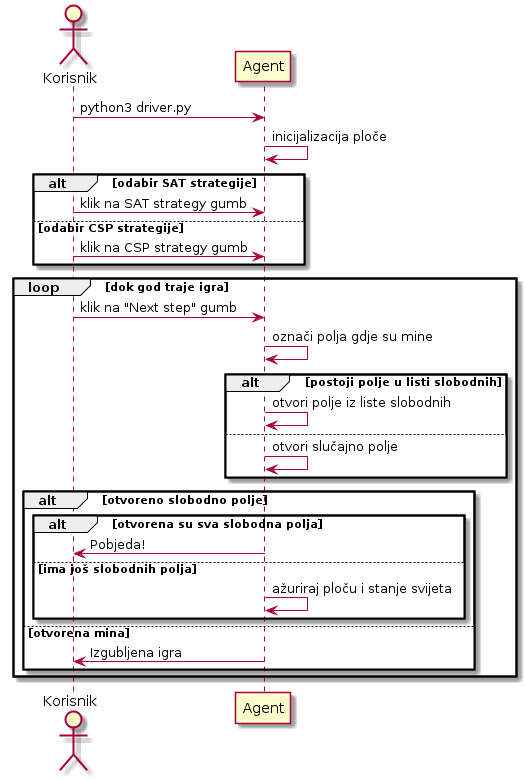
\includegraphics[width=\textwidth]{images/seq_diagram.png}
    \label{img:UML_komunikacijski}
    \caption{UML komunikacijski dijagram interakcije korisnika i aplikacije. Nakon što je
    igra završila korisnik ima opciju ponovno pokrenuti igru ili u potpunosti zatvoriti
    aplikaciju. Ta interakcija zbog konciznosti ovdje nije prikazana.}
\end{figure}

\subsection{SAT zaključivanje}

Algoritam SAT zaključivanja implicitno radi sa cijelim brojevima koji mogu biti pozitivni ili negativni, gdje pozitivan broj predstavlja istinitu vrijednost, a negativan broj lažnu. 
Ova strategija zato prikazuje svako polje ploče preko njegovog rednog broja te mu prilikom zaključivanja mijenja predznak. Sama vrijednost polja označava s 0 ili 1, pri čemu broj 1 označava da polje sadrži minu. 

Na početku, algoritam dobiva ograničenje koje govori koliko se ukupno mina nalazi na ploči. 
U svakom se koraku za svako novootvoreno polje generira ograničenje kao što je objašnjeno u
poglavlju \ref{sat} i dodaje u skup ograničenja. Zatim se za svako polje koje u tom trenutku
susjedno nekom otvorenom polju provjerava može li se sa sigurnošću reći da polje sadrži minu ili da
je prazno. Prvo se pretpostavi da je polje sigurno i ta se prepostavka dodaje u trenutnu bazu
znanja. Ako takav sustav nije zadovoljiv, sigurni smo da se na tome polju nalazi mina i polje se
označava. U suprotnom, pretpostavljamo da polje sadrži minu i gledamo zadovoljivost sustava. Ako on
nije zadovoljiv, polje je sigurno i dodaje se u skup polja za otvaranje.

Naposljetku se uzima jedno polje iz skupa sigurnih polja i otvara se. Također se otvaraju i sva susjedna polja ako niti jedno ne sadrži minu. Ako je skup sigurnih polja prazan, niti za jedno polje ne možemo sa sigurnošću reći da ne sadrži minu. Tada se otvara jedno slučajno odabrano neoznačeno polje s ploče.

\subsection{Simpleks metoda}

U ovoj strategiji svako je polje prikazano instancom razreda \textit{Variable} kako bi ih \textit{SimplexSolver} mogao obraditi i postavljati njihove vrijednosti. Vrijednost takve varijable implicitno može biti bilo koji decimalan broj.

Na samom početku izvođenja dodaje se ograničenje za svako polje, koje govori da vijednost tog polja mora nalaziti u skupu $[0, 1]$. Također, dodaje se ograničenje o ukupnom broju mina na ploči.

Dalje se u svakom sljedećem koraku generiraju ograničenja za svako novootvoreno polje na način opisan u poglavlju \ref{simplex}. 
\textit{SimplexSolver} automatski uzima u obzir sva dotadašnja ograničenja i mijenja vrijednosti varijabli kako bi sva ograničenja bila zadovoljena. Sva polja čija je vrijednost postavljena na 1 označavaju se kao mine. Za sva polja koja nisu označena s 1 smatra se da ne sadrže minu te se dodaju u skup polja za otvaranje. 

Na kraju se uzima slučajnim odabirom jedno polje iz tog skupa ili, ako je skup prazan, jedno slučajno odabarano polje iz cijele ploče. Odabrano polje se otvara, kao i susjedna ako niti jedno od njih ne sadrži minu, i korak strategije završava.

\section{Zaključak}

% ovdje možda ovaj odlomak? :
% Ovaj algoritam za razlučivanje ne ponaša se kao SAT postupak i to je očekivano. Glavna razlika između dva algoritma vidi se ukoliko algoritam nije siguran nalazi li se na nekom polju mina. SAT algoritam će tada pretpostaviti da se mina tamo nalazi i nikada neće otvoriti polje za koje ne može sa sigurnošću reći da nije mina. S druge strane, simpleks metoda takva polja dodaje u skup dostupnih polja te iz njega slučajnim odabirom odabire polje koje će otvoriti, što može biti i polje gdje se zapravo nalazi mina. Iz ovog razloga je SAT puno bolji algoritam za rješavanje ovog problema. Međutim, prednost simpleks algoritma nad SAT algoritmom je u vremenskoj složenosti.
\end{document}
